\let\negmedspace\undefined
\let\negthickspace\undefined
\documentclass[journal,12pt,twocolumn]{IEEEtran}
\usepackage{cite}
\usepackage{amsmath,amssymb,amsfonts,amsthm}
\usepackage{algorithmic}
\usepackage{graphicx}
\usepackage{textcomp}
\usepackage{xcolor}
\usepackage[justification=centering]{caption}
\usepackage{txfonts}
\usepackage{listings}
\usepackage{enumitem}
\usepackage{mathtools}
\usepackage{gensymb}
\usepackage{comment}
\usepackage[breaklinks=true]{hyperref}
\usepackage{tkz-euclide} 
\usepackage{listings}
\usepackage{gvv}                                        
\def\inputGnumericTable{}                                 
\usepackage[latin1]{inputenc}                                
\usepackage{color}                                            
\usepackage{array}                                            
\usepackage{longtable}                                       
\usepackage{calc}                                             
\usepackage{multirow}                                         
\usepackage{hhline}                                           
\usepackage{ifthen}                                           
\usepackage{lscape}

\newtheorem{theorem}{Theorem}[section]
\newtheorem{problem}{Problem}
\newtheorem{proposition}{Proposition}[section]
\newtheorem{lemma}{Lemma}[section]
\newtheorem{corollary}[theorem]{Corollary}
\newtheorem{example}{Example}[section]
\newtheorem{definition}[problem]{Definition}
\newcommand{\BEQA}{\begin{eqnarray}}
\newcommand{\EEQA}{\end{eqnarray}}
\newcommand{\define}{\stackrel{\triangle}{=}}
\theoremstyle{remark}
\newtheorem{rem}{Remark}
\begin{document}

\bibliographystyle{IEEEtran}
\vspace{3cm}

\title{10.5.4-5}
\author{EE23BTECH11033-killana jaswanth}
\maketitle
\newpage

\bigskip

\renewcommand{\thefigure}{\theenumi}
\renewcommand{\thetable}{\theenumi}
Question:\\
A small terrace at a football ground comprises of 15 steps each of which is 50
m long and built of solid concrete.Each step has a rise of 1/4 m and a tread of
1/2 m. Calculate the total volume of concrete required to build the terrace.
[Hint: Volume of concrete required to build the first step=\begin{align}
    V&=\frac{1}{4} \cdot \frac{1}{2} \cdot 50 
\end{align}
solution:
here\begin{table}[!ht]
 \centering
  \begin{tabular}{|c|c|c|}
\hline
\textbf{parameter}& \textbf{description}& \textbf{value}
\\\hline
\multirow{3}{1em}\\$l$&length&$50m$
\\\hline
$b$&breadth&$0.25m$
\\\hline
$h$&height&$0.5m$
\\\hline
$y(n)$& sum of volume&$6.25m^3$ 
\\\hline
\end{tabular}


   \caption{formula parameters}
   \label{tab:10.5.4.5}
   \end{table}
\begin{align}
x\brak{Z}&=\frac{x(0)}{1-\,z^{-1}}+\frac{dz^{-1}}{\brak{1-{z^{-1}}}^2}\:\:
\quad\abs{z}>\abs{1}\\
x\brak{Z}&=\frac{6.25}{1-\,z^{-1}}+\frac{6.25z^{-1}}{\brak{1-{z^{-1}}}^2}\:\:\quad\abs{z}>\abs{1}\\
&=\brak{\frac{6.25}{\brak{1-z^{-1}}^2}} \quad\abs{z}>\abs{1}\\
\end{align}
\begin{figure}[!ht]
    \centering
    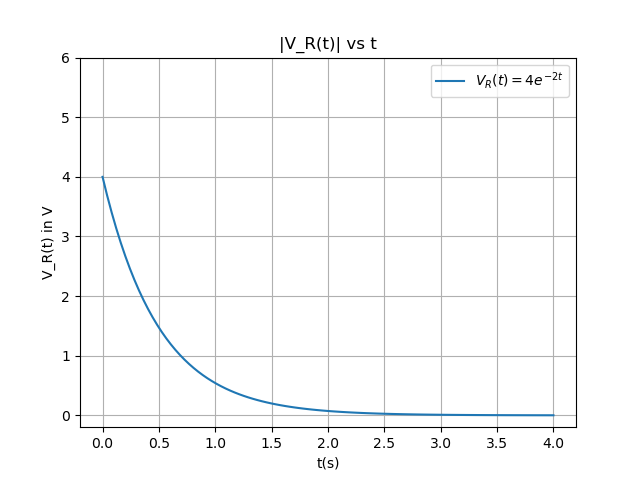
\includegraphics[width=1\linewidth]{fig.png}
    \caption{plot x\brak{n} vs n}
    \label{fig:enter-label}
\end{figure}
convolution for y\brak{n}:\\
\begin{align}
Y\brak{n}&=x\brak{n}*u\brak{n}\\
Y\brak{Z}&=x\brak{Z}U\brak{Z}\\
U\brak{Z}&=\frac{1}{1-\,z^{-1}}\quad\abs{z}>\abs{1}\\
Y\brak{Z}&=\brak{\frac{6.25}{1-\,z^{-1}}+\frac{6.25z^{-1}}{\brak{1-{z^{-1}}}^2}}\brak{\frac{1}{1-\,z^{-1}}}\quad\abs{z}>\abs{1}\\
Y\brak{z}&=\frac{6.25}{\brak{1-z}^{-3}} \quad\abs{z}>\abs{1}\\
\end{align}
  contour integration to find inverse z transform
\begin{align}
y(15)&=\frac{1}{2{\pi}j}{\oint_c}Y\brak{Z}z^{14}dz\\
&=\frac{1}{2{\pi}j}{\oint_c}{\frac{6.25z^{14}}{\brak{1-z^{-1}}^{3}}}\\
\end{align}
pole at 1 repeated 3 times\\
\begin{align}
m&=3\\
R&=\frac{1}{\brak{m-1}!}\lim_{z\to a}\frac{d^{m-1}}{dz^{m-1}}\brak{\brak{z-a}^mf{\brak{z}}}\\
&=\frac{1}{\brak{2!}}\lim_{z\to 1}\frac{d^2}{dz^2}\brak{\brak{z-1}^{3}\frac{6.25z^{16}}{\brak{z-1}^3}}\\
&=3.125\lim_{z\to1}\frac{d^2}{dz^2}\brak{z^{16}}\\
y\brak{15}&=750
\end{align}
 \end{document}
